\section{一次成像现象}
\label{sec:one-shot}

本节介绍了 One-Shot OPD 的实验设置与结果。我们研究了 \textit{single query 能够恢复 full-data OPD 的多少收益，以及该收益的鲁棒性如何}。

\begin{tcolorbox}[takeawaysbox]
\textbf{一次查询即可引发稳健的OPD收益。}
单次查询即可在任务领域和模型族之间恢复大部分教师-学生差距。该收益对查询难度、响应长度和采样温度均不敏感，即使学生从未解决过的查询，其效果也与总是能解决的查询相当。
\end{tcolorbox}

\subsection{实验设置}
\label{sec:setup}

我们建立了一次性OPD，涵盖数学、代码生成、指令遵循和智能体工具使用，以进行受控分析，测试其通用性。

\paragraph{模型}

\begin{table}[t]
\centering
\small
\caption{
实验中使用的师生配对。
}
\label{tab:full}
\setlength{\tabcolsep}{5pt}
\renewcommand{\arraystretch}{1.12}
\begin{tabularx}{\textwidth}{@{}lXX@{}}
\toprule
\textbf{Setting} & \textbf{Student} & \textbf{Teacher} \\
\midrule

\multirow{3}{*}{Mathematical reasoning}
& DeepSeek-R1-Distill-Qwen-1.5B\newline
{\footnotesize (R1-Distill-1.5B)}
& JustRL-DeepSeek-1.5B\newline
{\footnotesize (JustRL-1.5B)} \\

& Llama-3.2-3B-Instruct\newline
{\footnotesize (Llama-3B-It)}
& GT-Llama-3.2-3B-Instruct-MATH\newline
{\footnotesize (GT-Llama-3B-Math)} \\

& OLMo-3-7B-Instruct-DPO\newline
{\footnotesize (OLMo-7B-It-DPO)}
& OLMo-3-7B-Instruct\newline
{\footnotesize (OLMo-7B-It)} \\

\midrule

Code generation
& DeepSeek-R1-Distill-Qwen-1.5B\newline
{\footnotesize (R1-Distill-1.5B)}
& Nemotron-Research-Reasoning-Qwen-1.5B-v2-RLVE\newline
{\footnotesize (Nemotron-1.5B)} \\

Instruction following
& DeepSeek-R1-Distill-Qwen-1.5B\newline
{\footnotesize (R1-Distill-1.5B)}
& UltraData-IF-1.5B \\

Agentic tool use
& Qwen2.5-Coder-1.5B-Instruct\newline
{\footnotesize (Qwen-Coder-1.5B)}
& Hammer2.1-1.5b\newline
{\footnotesize (Hammer-1.5B)} \\

\bottomrule
\end{tabularx}
\end{table}

对于每个领域，我们将一个学生模型与同家族的微调后教师模型配对。表~\ref{tab:full} 列出了完整的标识符以及全文中使用的简称。数学、代码生成和指令遵循任务共享同一个学生模型 R1-Distill-1.5B \citep{deepseekai2025deepseekr1incentivizingreasoningcapability}，其对应的教师模型分别为 JustRL-1.5B \citep{he2025justrl}、Nemotron-1.5B \citep{zeng2025rlve}，以及我们从同一学生模型微调得到的一个指令遵循变体（见附录~\ref{app:IF-setup}）。在 Agentic 工具使用场景中，学生模型为 Qwen-Coder-1.5B \citep{hui2024qwen2}，教师模型为 Hammer-1.5B \citep{lin2024hammer}。为了检验该现象是否仅针对基于 Qwen 的模型对，我们还引入了来自其他家族的两个数学推理模型对：Llama-3B-It \citep{grattafiori2024llama} 与 GT-Llama-3B-Math \citep{zhang2025co}，以及 OLMo-7B-It-DPO 与 OLMo-7B-It \citep{olmo2025olmo}。

\paragraph{数据集}
领域特定的训练集包括用于数学推理的DAPO-Math-17K \citep{yu2026dapo}、用于代码生成的Open-R1 Codeforces \citep{penedo2025codeforces}、用于指令遵循的UltraData-SFT-2605 \citep{ultradata-sft-2605}的采样子集，以及用于智能体工具调用的xLAM-function-calling-60K \citep{liu2024apigen}。对于数学领域的one-shot OPD，我们选取了三个查询，覆盖简单、中等和困难三种初始难度，其得分基于学生在训练前8次滚动测试中的通过率（分别对应\(8/8\)、\(4/8\)和\(0/8\)）。在其他领域中，one-shot查询则从相应训练集中随机采样。附录~\ref{app:model-data}详细介绍了数据集预处理过程及所选的one-shot查询。

\paragraph{训练}
我们在 \texttt{veRL} \citep{sheng2025hybridflow} 中实现了 OPD。  
本节的数学推理运行优化公式~\ref{eq:topk-advantage} 的前-\(k\) 优势，使用 \(k=16\)；代码、指令遵循和 Agentic 运行则优化公式~\ref{eq:token-advantage} 的采样 token 优势。  
每次更新均使用 $64$ 次 rollout 构成的批量。我们采用 AdamW 优化器，学习率为 $10^{-6}$，rollout 温度为 $1.0$，梯度裁剪范数为 $1.0$；其余超参数列于表~\ref{tab:opd-hyperparams} 中。


\paragraph{评估。}
对于数学任务，我们在 MATH-500 \citep{hendrycksmath2021}、AMC 2023 \citep{li2024numinamath} 和 AIME 2025 \citep{balunovic2026matharena} 上进行评估，每个问题采样 16 个响应，并报告 avg@16 准确率。  
对于代码生成任务，LiveCodeBench v6 (LCB v6) \citep{jain2025livecodebench} 每个问题使用 3 个采样解法，并通过官方基于执行的评估器报告 avg@3 得分。  
对于指令遵循任务，Multi-IF \citep{he2024multi} 评估三轮对话，并报告其八种语言上最终一轮的平均得分。  
对于 Agentic 工具使用任务，BFCL v3 \citep{patil2025bfcl} 报告所评估子集上的 avg@8 得分。响应长度上限分别为：\(31{,}744\) token 用于数学任务，\(65{,}536\) token 用于 LCB v6，\(16{,}384\) token 每轮用于 Multi-IF，以及 \(4{,}096\) token 用于 BFCL v3。除非另有说明，数学任务的结果报告的是在 MATH-500、AMC 2023 和 AIME 2025 上验证准确率的宏平均值，虚线标记教师模型表现。


\begin{figure}[t]
  \centering
  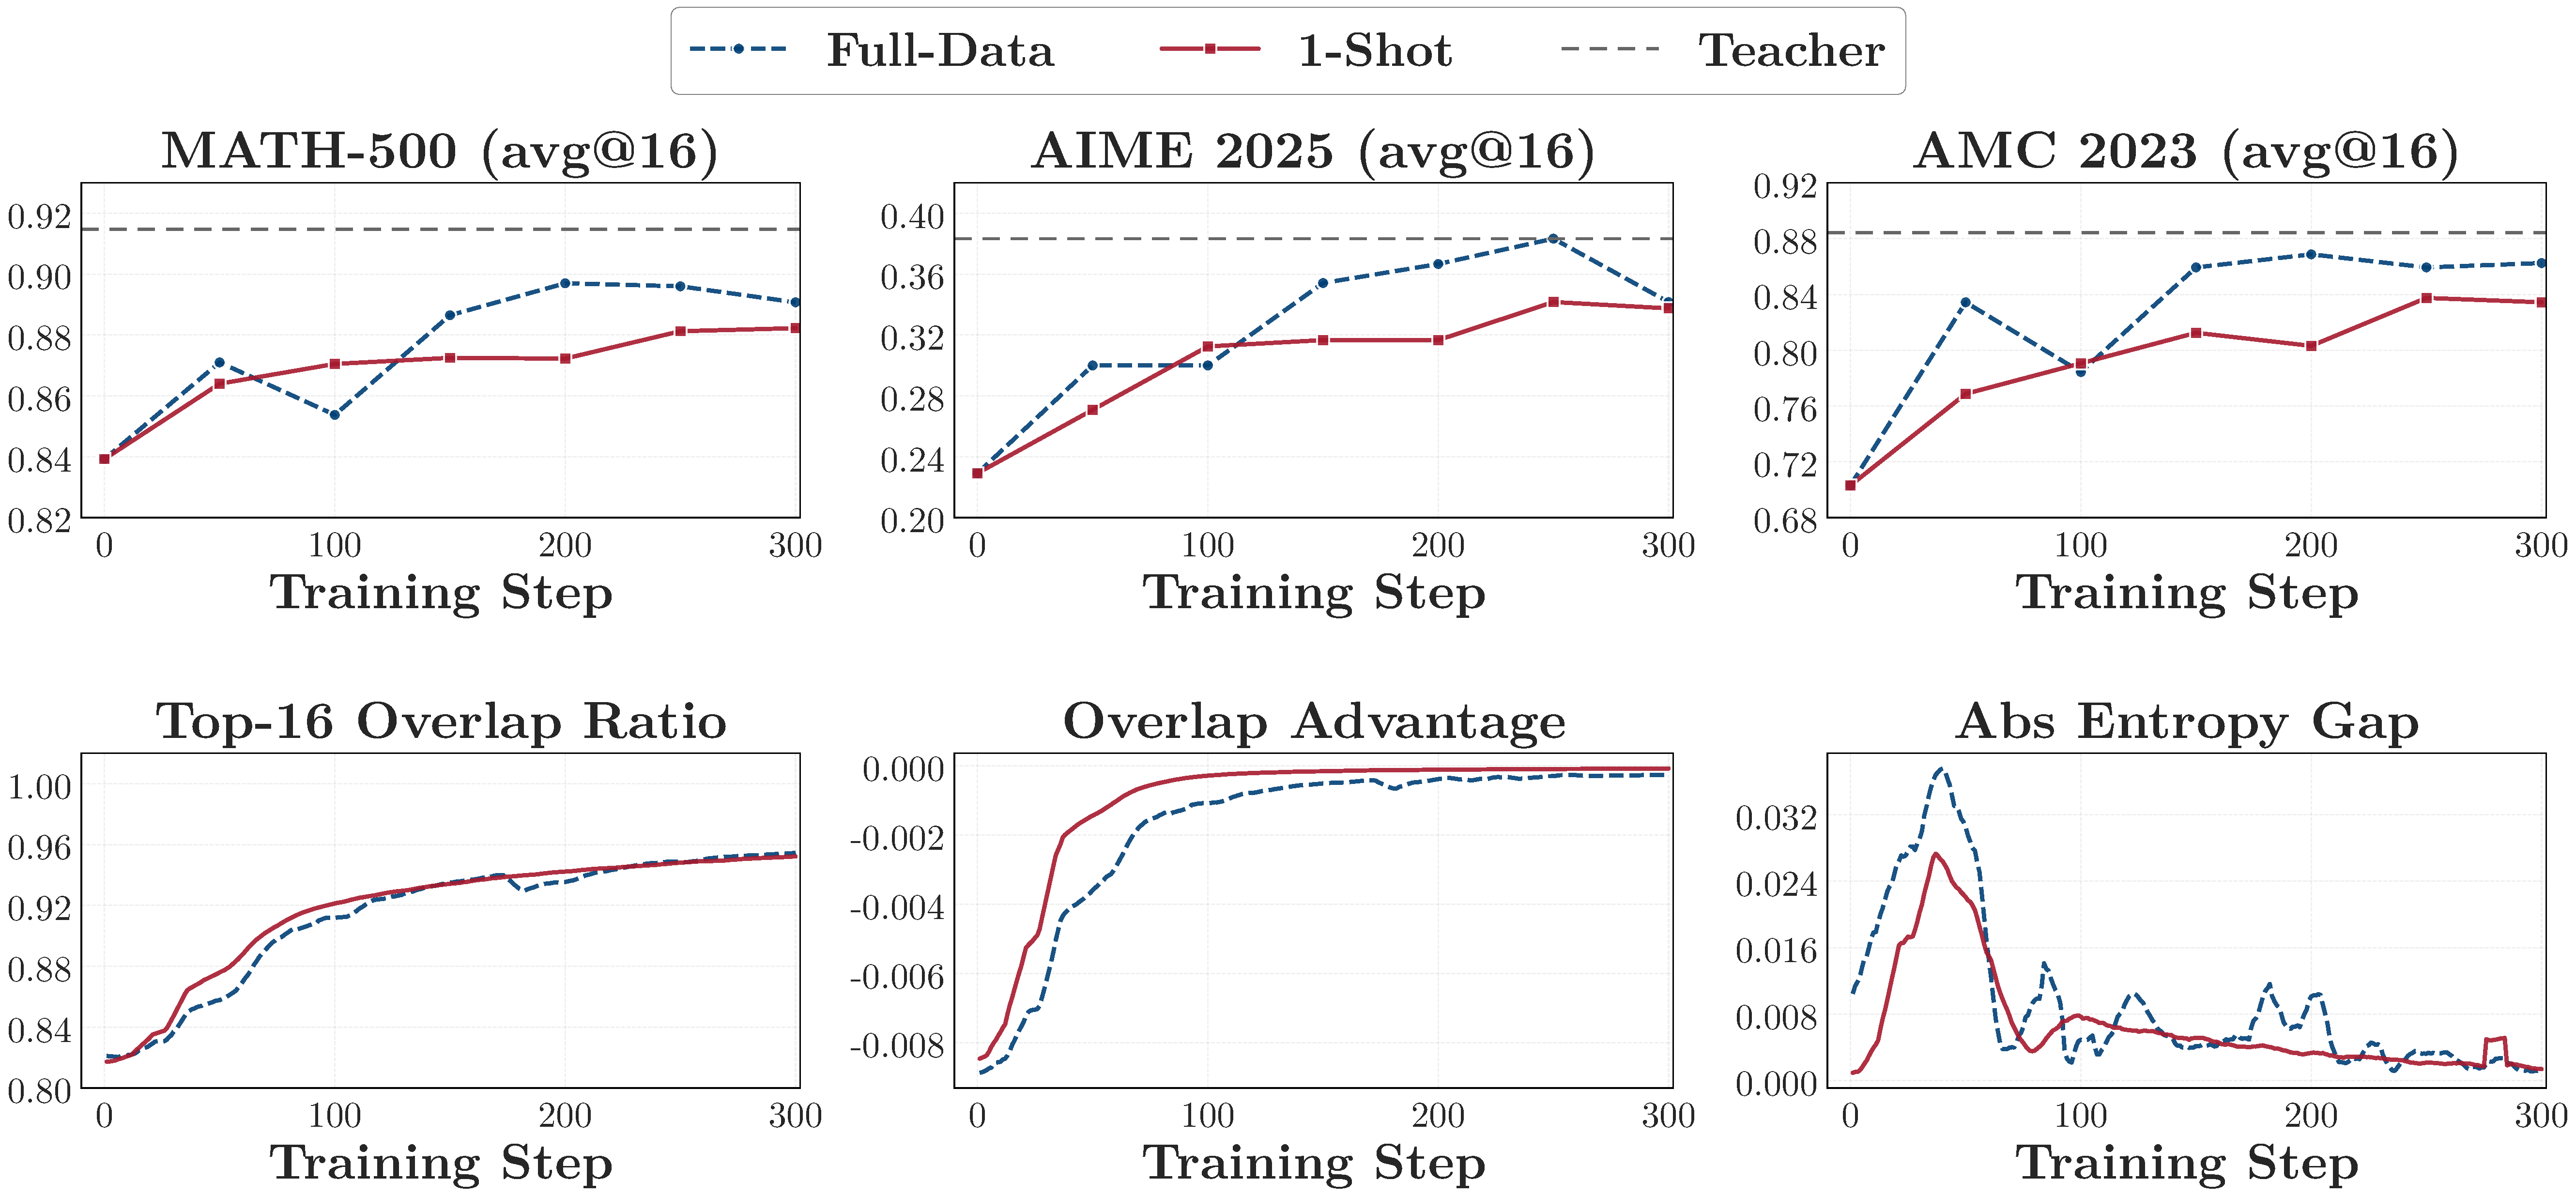
\includegraphics[width=\textwidth]{figures/3_oneshot_math300.pdf}
  \caption{one-shot OPD 在数学推理上的验证准确率和训练动态。}
  \label{fig:math_oneshot_dynamics}
\end{figure}

\begin{figure}[t]
  \centering
  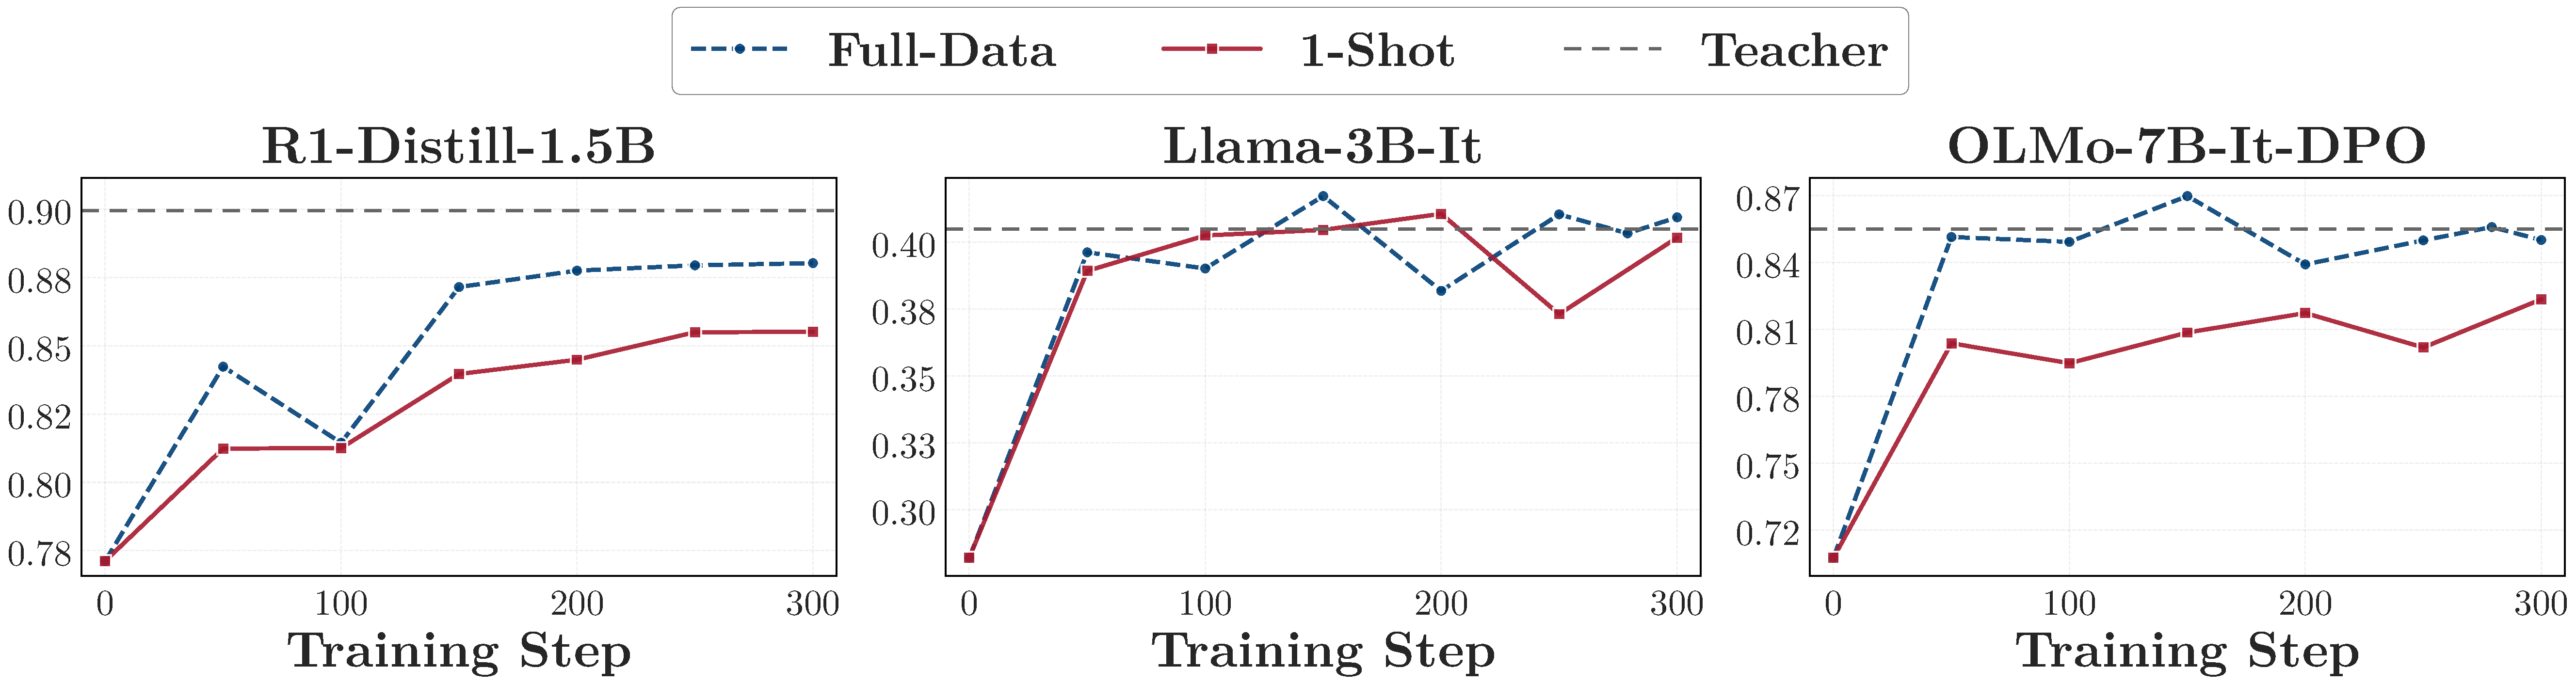
\includegraphics[width=\textwidth]{figures/3_cross_family.pdf}
  \caption{
  在数学推理任务上，对三个学生-教师模型族进行one-shot OPD的验证准确率，结果为MATH-500和AMC 2023的平均值。由于Llama模型对AIME 2025的得分接近零，因此该数据集被排除。
  }
  \label{fig:cross_family}
\end{figure}

\begin{figure}[t]
  \centering
  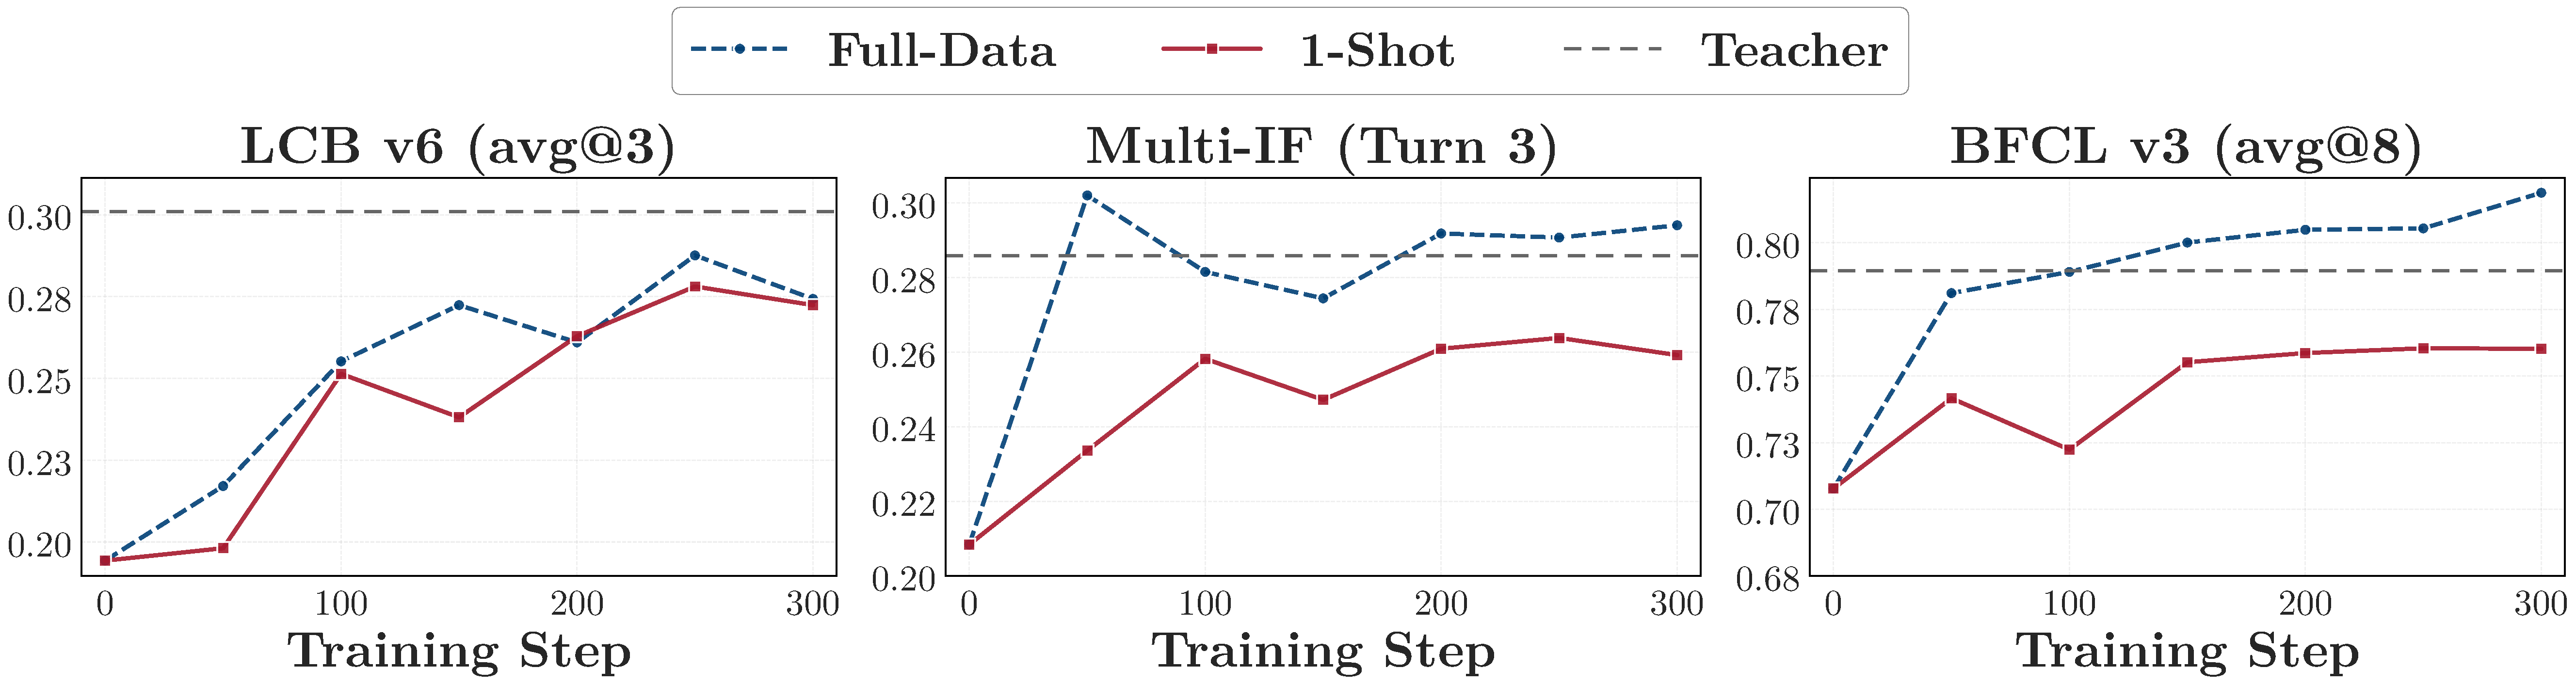
\includegraphics[width=\textwidth]{figures/3_cross_domain.pdf}
  \caption{
  one-shot OPD 在三个任务领域中的验证准确率。
  }
  \label{fig:cross_domain}
\end{figure}

\begin{figure}[t]
  \centering
  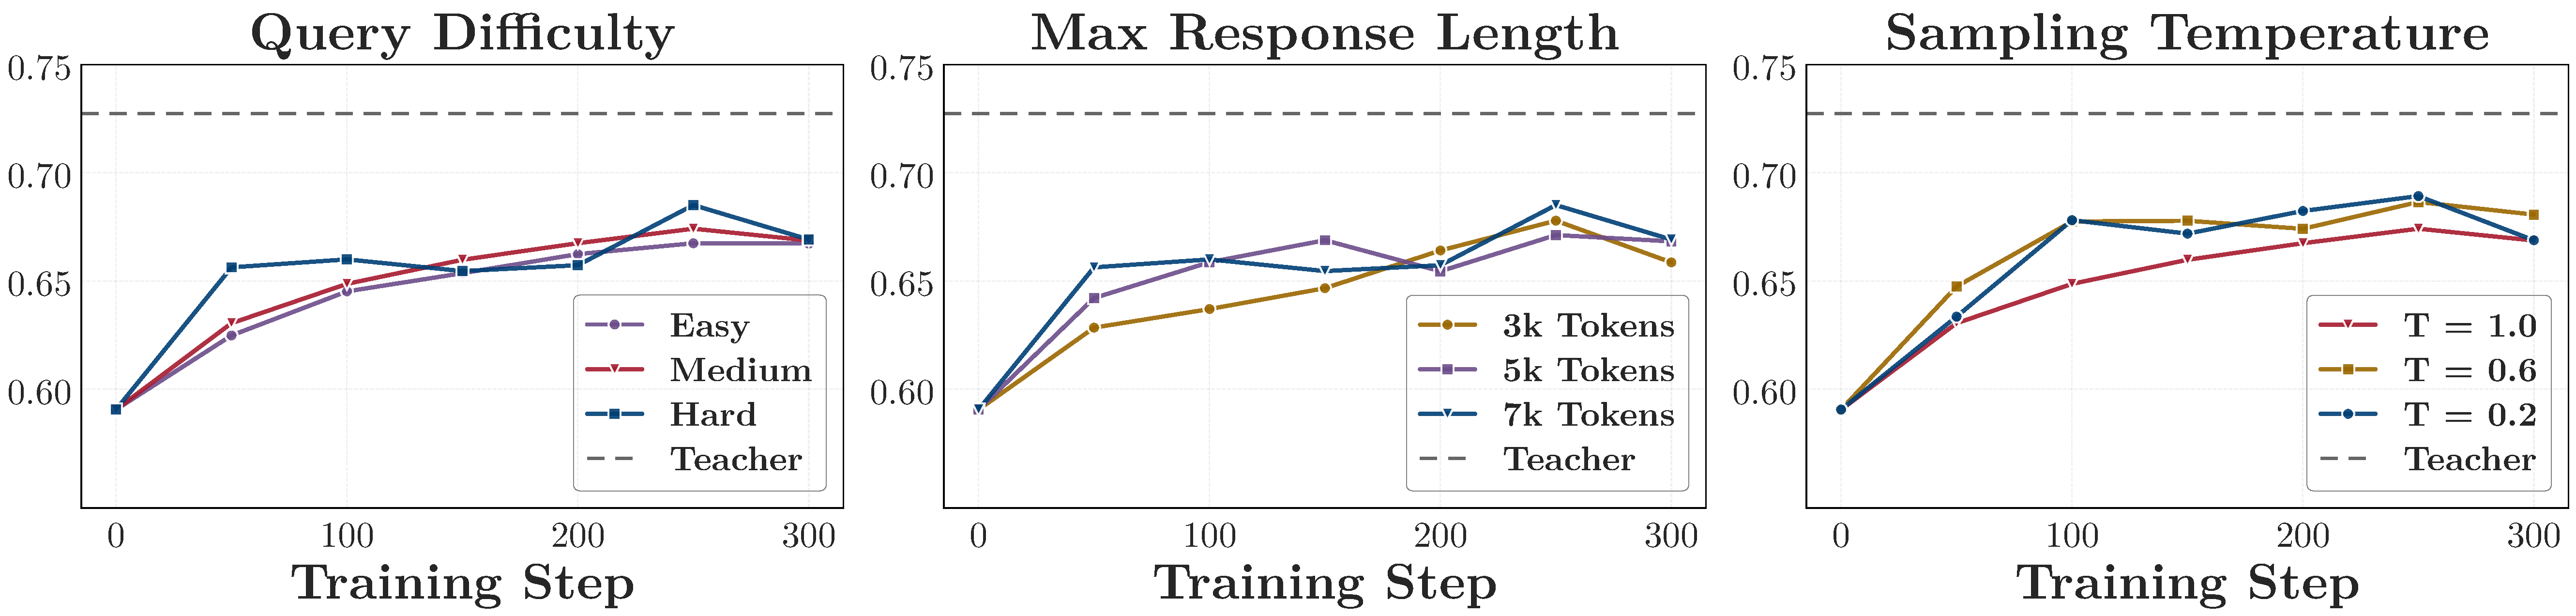
\includegraphics[width=\textwidth]{figures/3_ablations.pdf}
  \caption{
  在不同查询难度、硬查询的响应长度限制以及中等查询的采样温度下，one-shot OPD 的验证准确率。
  }
  \label{fig:probe_prompt}
\end{figure}


\subsection{实验结果}
\label{sec:finding-recovery}

\paragraph{One-shot OPD 在数学上恢复了大部分全数据 OPD 的增益。}

图~\ref{fig:math_oneshot_dynamics} 表明，在单个查询上进行训练可提升在 MATH-500、AIME 2025 和 AMC 2023 上的准确率，使其在所有三个基准上均接近全数据 OPD。三者平均来看，one-shot OPD 达到 \(68.5\) ，而全数据 OPD 为 \(69.8\) ，恢复了教师-学生差距的 \(69\%\) ，以及全数据 OPD 在第 300 步时增益的 \(87\%\) 。超过第 \(300\) 步后，两条曲线始终维持在约 \(3\) 个点的范围内，恢复比例从 \(62\%\) 到 \(89\%\) ，持续至第 \(1000\) 步，此时 one-shot OPD 达到 \(68.4\) 对比 \(72.1\) ，恢复了全数据 OPD 增益的 \(72\%\) （图~\ref{fig:teaser}）。在两种情景下，训练动态遵循相同的对齐过程：top-16 重叠率上升至全数据水平，重叠 token 优势趋近于零，绝对熵差几乎完全闭合。因此，即使所有回溯轨迹均源自单一查询，OPD 仍能提升准确率，并逐步将学生分布与教师在访问状态上的分布对齐。


\paragraph{one-shot效应在不同家族和任务领域中均具有鲁棒性。}
\label{sec:one-shot-robust}
图~\ref{fig:cross_family} 表明，one-shot OPD 在所有三个学生-教师模型族中均提升了数学推理能力。在最终检查点，平均得分分别从对应的学生基准的 \(77.1\) 、\(28.2\) 和 \(70.8\) 提升至 R1-Distill-1.5B、Llama-3B-It 和 OLMo-7B-It-DPO 的 \(85.5\) 、\(40.2\) 和 \(82.4\) 。图~\ref{fig:cross_domain} 进一步表明，该效果不仅限于数学推理：在代码生成、指令遵循和 Agentic 工具使用任务上，one-shot OPD 分别恢复了 \(73\%\) 、\(66\%\) 和 \(64\%\) 的相应教师-学生差距。综上所述，这些结果表明，one-shot 效应在模型族和任务领域之间均具有鲁棒性。


\paragraph{one-shot 效应对于查询和展开特性具有鲁棒性。}

我们接下来考察在不同查询难度、响应长度预算以及轨迹采样温度下，one-shot OPD 是否依然有效。如图~\ref{fig:probe_prompt} 所示，无论查询是简单、中等还是困难，one-shot OPD 均能发挥作用，尽管三种情景下正确轨迹的比例演化方式差异显著（附录~\ref{app:training-accuracy}）：简单查询几乎每一步都能解决，中等查询在训练过程中逐渐变得可解，而困难查询始终无法解决。收紧响应长度上限和降低轨迹采样温度均能保持 one-shot 的优势。综合来看，这些结果表明，one-shot OPD 对查询难度、响应长度预算以及轨迹采样温度具有鲁棒性。
